\documentclass[tikz,border=10pt]{standalone}
\usepackage{tikz}
\usetikzlibrary{matrix}

\begin{document}
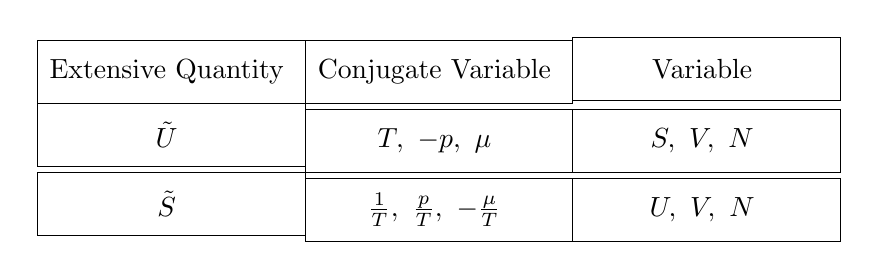
\begin{tikzpicture}
\matrix (m) [
    matrix of nodes,
    nodes in empty cells,
    nodes={draw, minimum height=0.8cm, minimum width=3.4cm, align=center},
    column sep=-\pgflinewidth,
    row sep=-\pgflinewidth
] {
    {Extensive Quantity} & {Conjugate Variable} & {Variable} \\
    $\tilde{U}$ & $T,\ -p,\ \mu$ & $S,\ V,\ N$ \\
    $\tilde{S}$ & $\frac{1}{T},\ \frac{p}{T},\ -\frac{\mu}{T}$ & $U,\ V,\ N$ \\
};
\end{tikzpicture}
\end{document}
